\providecommand{\relativeRoot}{../..}
\documentclass[\relativeRoot/main.tex]{subfiles}
\graphicspath{
    {\subfix{./figures/}}
}


\begin{document}

\section{Lymphatic Metastatic Progression}
\label{sec:intro:lymph_spread}

The lymphatic system is a vascular network that is imbued in most human tissue alongside the circulatory system (except e.g. the brain). It consists of thin-walled capillaries that are more permeable than blood vessels. Extracellular fluid, with which cells are provided by circulatory vessels, and into which they release waste products, drains into these permeable lymphatic capillaries and is transported back into the blood stream at the \emph{thoracic duct} \cite{willard-mack_normal_2006,wissmann_pathways_2006,oliver_rediscovery_2002}.

Also included in the lymphatic system are organs and structures that play an important role in the human immune response. For example, the lymph nodes, which are located at numerous junctions of afferent lymphatic vessels (a schematic is provided in \cref{fig:intro:lymph-node}). The incoming fluid flows through a dense, sponge-like labyrinth where the particles it carries are brought into contact with various cells of the immune system (e.g. \emph{lymphocytes} and \emph{macrophages}). Eventually, it drains into the efferent lymphatic vessel at the \emph{hilus} of the lymph node \cite{willard-mack_normal_2006,ohtani_structure_2008}.

\begin{figure}
    \begin{minipage}[c]{0.6\textwidth}
        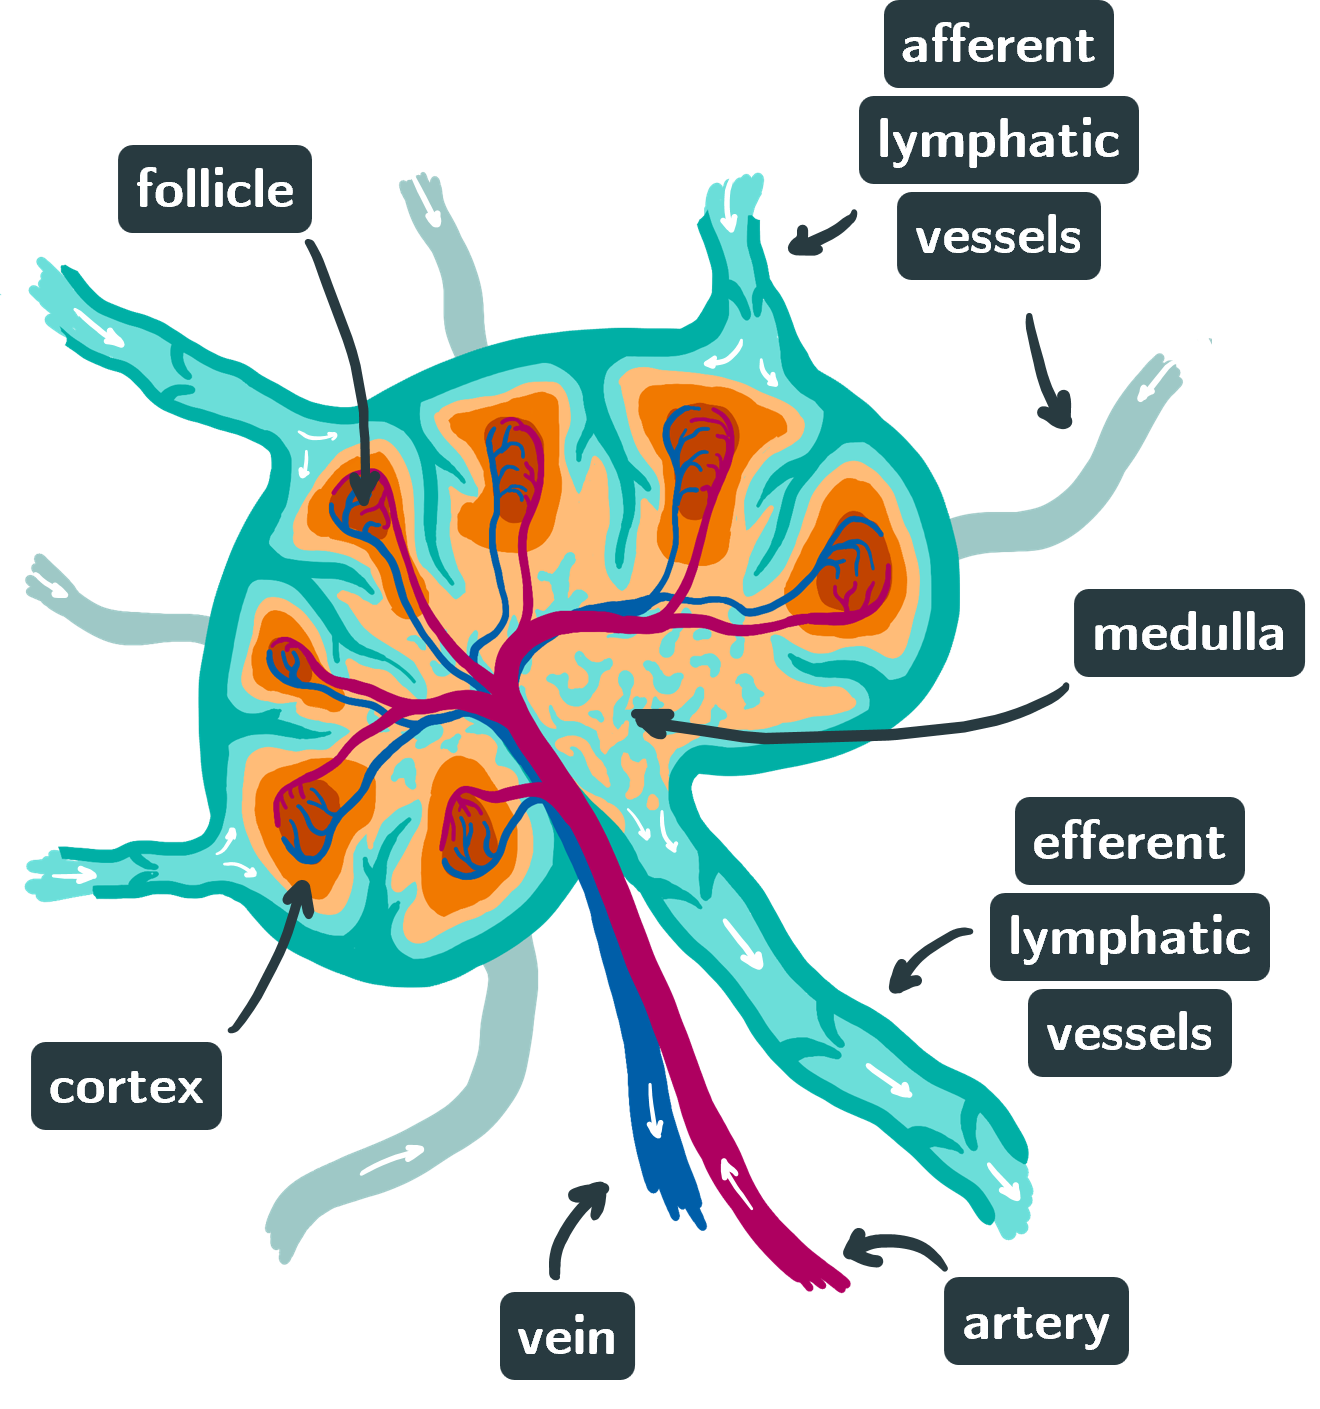
\includegraphics[width=\textwidth]{figures/lymph-node_labelled.png}
    \end{minipage}
    \hfill
    \begin{minipage}[c]{0.38\textwidth}
        \caption[
            Lymph node schematic
        ]{
            Schematic drawing of a lymph node. Lymph fluid from the \emph{afferent} lymphatic vessels spreads into the \emph{subcapsular sinuses} (following the white arrows) down along the \emph{lateral transverse sinuses} through a dense labyrinth into the \emph{medullary sinuses} (all shown in light green in the main node) where it finally exits the lymph node at the \emph{hilus} through the \emph{efferent} lymphatic vessel. Over the vast surface are of this labyrinth, various immune cells -- located in the \emph{cortex} and \emph{follicle} -- can interact with the contents of the lymph fluid \cite{willard-mack_normal_2006,ohtani_structure_2008}.
        }
    \end{minipage}
    \label{fig:intro:lymph-node}
\end{figure}

The human lymphatic system contains several hundred lymph nodes \cite{willard-mack_normal_2006} and since they are not distributed in the exact same way in all humans, they are often categorized into \glspl{lnl}. For the head and neck region, this categorization emerged to standardize first \glspl{nd} \cite{robbins_standardizing_1991} and later \gls{rt} \cite{gregoire_ct-based_2003}. The boundaries of these \glspl{lnl} were defined to be easily identifiable during surgery or on \gls{ct} scans and hence consist of bones, muscles, blood vessels or nerves. In \cref{fig:intro:schematics_head} we show a sketch of the \glspl{lnl} in the head and neck region. This is described in much more detail e.g. by \citeauthorandlink{lengele_anatomical_2007} or by \citeauthorandlink{gregoire_delineation_2014}.

An \gls{hnscc} tumor may shed live cells into the lymph fluid, from where, following the drainage through a lymphatic vessel, they enter a lymph node. In contrast to normal epithelial cells, those of \glspl{scc} exhibit factors that suppress \emph{anoikis}, a form of programmed cell death initiated when these cells become detached from their surroundings \cite{peltanova_effect_2019}. Consequently, these live cells detached from the tumor may start to proliferate inside a lymph node when they get stuck in its dense pathways and are not destroyed by the immune response inside the node.

Once a metastasis has formed inside a lymph node, this new lesion itself may again shed tumor cells that can flow further downstream where they, too, start to grow. It is not clear whether this process must happen stepwise, i.e. that lymph nodes must become involved in the order they appear in their lymphatic chain, or if tumor cells may pass through lymph nodes. In case they can traverse a lymph node, that would result in ``skip lesions'' which are in fact observed \cite{woolgar_topography_2007}, but they may also stem from direct spread originating in the main tumor.

Presence of lymph node metastasis is linked to a significantly lower survival of \gls{hnscc} patients and hence it is considered one of the most prognostic factors \cite{jones_level_1994,lim_distributions_2006,takes_staging_2004}.

\begin{figure}
    \centering
    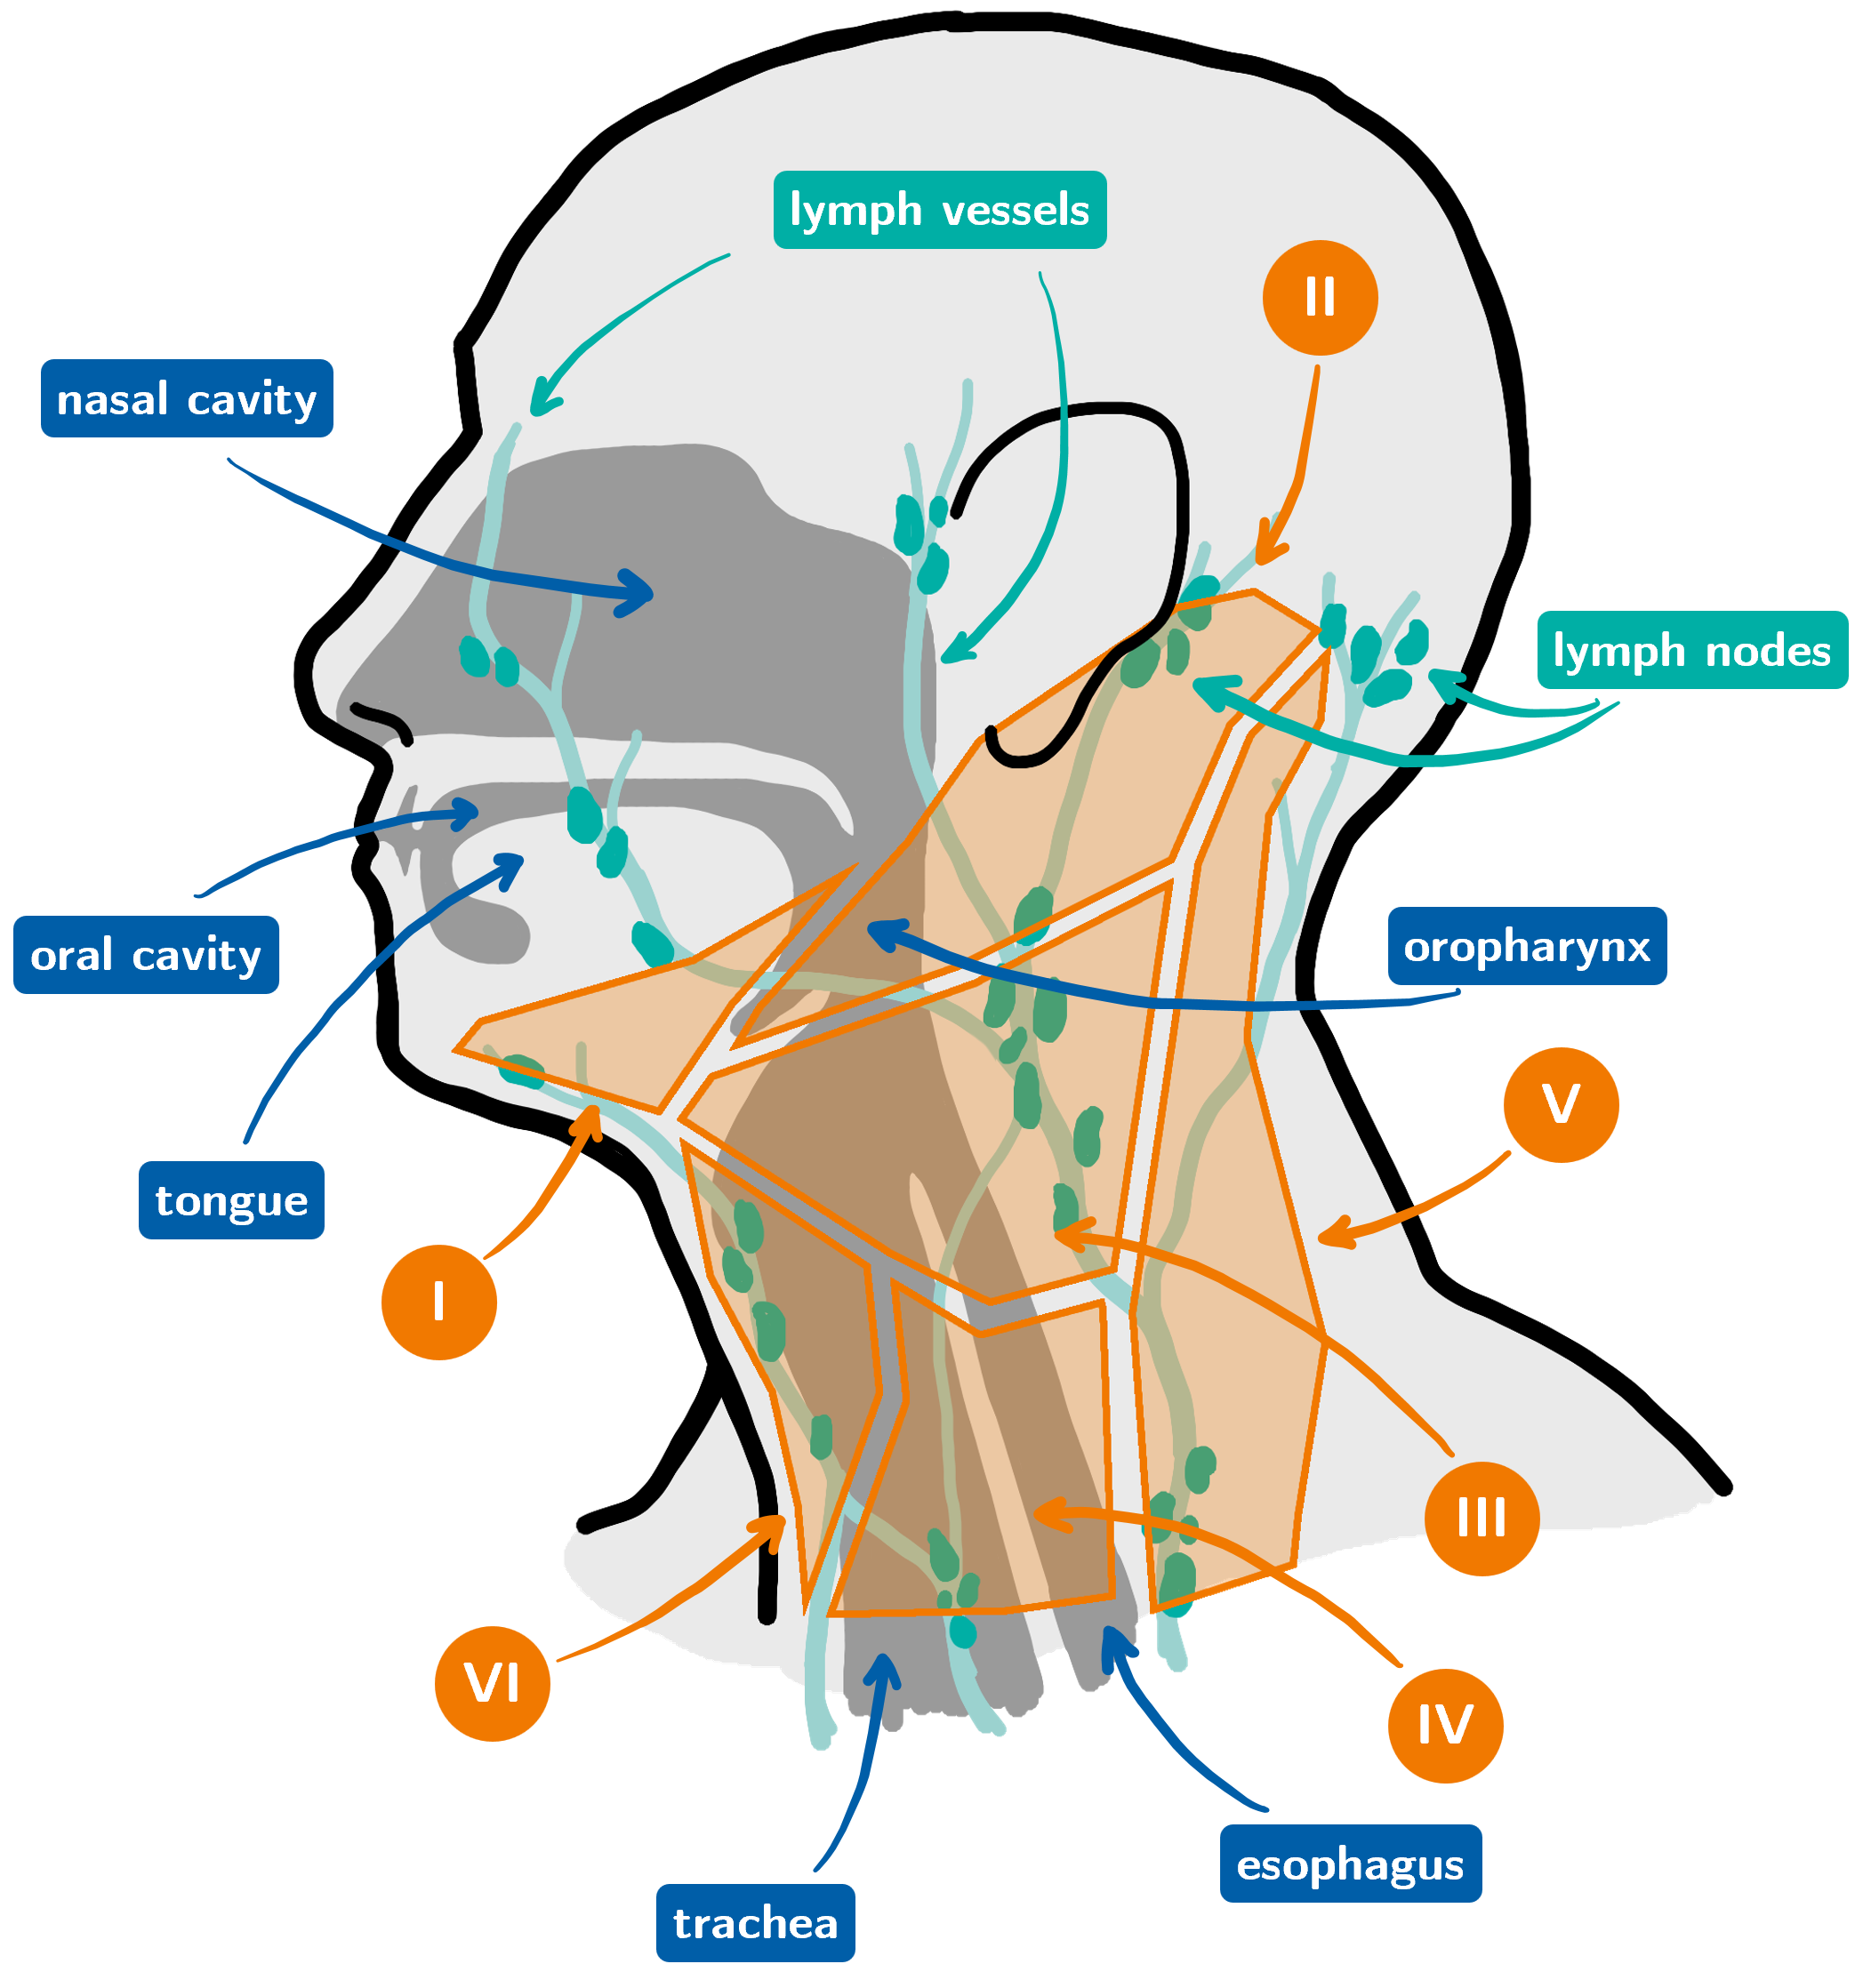
\includegraphics[width=\textwidth]{figures/head_and_neck_labelled.png}
    \caption[
        Schematic drawing of the head and neck region.
    ]{
        Schematic drawing of the lymphatic network in the head and neck region. The shaded area in dark gray depicts a sagittal cross-section of the upper respiratory track and is labelled with blue arrows and tags. Lymphatic vessels are drawn in light green with dark green lymph nodes attached to them. On top, using a transparent shade of orange and orange outlines, we have roughly indicated the location of the \glspl{lnl}. They group the lymph nodes in the head and neck region into regions that are separated by anatomical features not shown in this schematic. E.g., the inferior border of the hyoid bone separates \gls{lnl} II and III axially. The diagram is based on the anatomical illustrations in \citeauthorandlink{lengele_anatomical_2007} and has been adapted for this chapter.
    }
    \label{fig:intro:schematics_head}
\end{figure}

\end{document}
